\chapter{Terminology Preliminaries}\label{ch:prelim}
In this chapter, we will introduce the core definitions used in this thesis. 
Most of the definitions of graph theory are taken from Diestel \cite{Diekert2005}. 
For definitions in the area of \textit{parametrized complexity}, the book by Cygan et al. \cite{Cygan2015} gives a very good introduction.

%% TODO State Draft
Continuing an intensive study of parametrized complexity of that problem. 

\section{Graph Theory}
% In 1736, Euler Örst introduced the notion of graph theory. In the history of mathematics, the solution given by Euler of the well known Konigsberg bridge problem is
%kconsidered to be the Örst theorem of graph theory. This has now become a subject
%kgenerally regarded as a branch of a combinatorics. The theory of graph is an extremely
%kuseful tool for solving combinatorial problems in di§erent areas such as geometry, algebra, number theory, topology, operations research, optimization and computer science.

We quickly state the following definitions given by {\cite[p.~xxx]{diestel10}}.

%% TODO Path, Subgraph, Induced Subgraph, Copnnected 
\begin{definition}[Graph {\cite[p. 3]{diestel10}}]
    A graph is a pair $G = (V, E)$ of two sets where $V$ denotes the vertices and $E \subseteq V \times V$ the edges of the graph.  A vertex $v \in V$ is incident with an edge $e \in E$ if $v \in e$. Two vertices $x, y$ are adjacent, or neighbours, if $\{x,y \} \in E$.
    % Size of the Graph?
\end{definition}

%TODO Quote
\begin{definition}[Vertex Degrees]
    The \textit{degree} $d_G(v)$ (If G is clear, also $d(v)$) of a vertex $v$ is the number of neighbors of v. We call a vertex of degree 0 as isolated and one of degree 1 as a pendant.
\end{definition}

\begin{definition}[isomorphic Graphs, {\cite*[p. 3]{diestel10}}]
Let \G and $G' = (V', E')$ be two graph. We call $G$ and $G'$ \underline{isomorphic}, if there exists a bijection $\phi: V \rightarrow V'$ with $\{x, y\} \in E \Leftrightarrow \phi(x)\phi(y) \in E'$ for all  $x,y \in V$. Such a map $\phi$ is called \underline{isomorphism}.
\end{definition}
If a graph $G$ is isomorphic to another graph $h$, we denote $G \simeq H$. 

\begin{definition}[Special Graph Notations {\cite[p.~27]{diestel10}}]
    A simple Graph
    
    A directed Graph is a graph
    
    A Multi Graph
    
    A Planar Graph
\end{definition}

% TODO Quote e.g. The open neighborhood number of a graph
\begin{definition}[Closed and Open Neighborhoods {\cite{Balakrishnan2012}}]
    Let \G be a (non-empty) graph. 
    The set of all neighbors of $v$ is the \underline{open neighborhood} of $v$ and denoted by $N(v)$; the set $N[v] = N(v) \Cup \{v\}$ is the \underline{closed neighborhood} f $v$ in $G$. When G needs to be made explicit, those open and closed neighborhoods are denoted by $N_G(v)$ and $N_G[v]$. 
\end{definition}

\begin{definition}[Subgpraph and Induced Subgraph]
    asd
\end{definition}

\begin{definition}[Isomorphic Graph]
    asd
\end{definition}

\subsection*{Graph Classes}

We call the class of graphs without any special restrictions ``General Graphs''.

\begin{definition}[r-partite Graphs]
    Let $r \geq 2$ be an integer. A Graph $G = (V,E)$ is called ``r-partite'' if V admits a partition into r classes such that every edge has its ends in different classes: Vertices in the same partition class must not be adjacent. 
    
    For the case $r = 2$ we say that the G is ``bipartite'' 
    %      %        TODO mage of a bipartite Graph
    
\end{definition}

\begin{definition}[Chordal Graphs]
    
\end{definition}

\begin{definition}[Split Graphs]
    
\end{definition}

\begin{definition}[Path Graph $P_i$]
    
\end{definition}

\begin{definition}[Bipartite Graph, {\cite[p.5]{Bondy2008}}]
    
A \textit{\bg} is a Graph G whose vertex set can be partitioned into two subsets X and Y, so that each edge has one end in X and one end in Y. Such a partition (X,Y) is called a \textit{bipartition} of G.

\end{definition}


\begin{definition}[Planar Graphs {\cite[Chapter 4]{diestel10}}]

A \textit{plane graph} is a pair $(V,E)$ of finite sets with the following properties:

\begin{itemize}
    \item $V \subseteq \mathbb{R}^2$ (Vertices)
    \item Every edge is an arc between two vertices 
    \item different edges have different sets of endpoints
    \item The interior of an edge contains no vertex and no point of any other edge
\end{itemize}

An embedding in the plane, or \textit{planar embedding}, of an (abstract) graph $G$ is an isomorphism between $G$ and a plane graph $H$. A \textit{plane graph} can be seen as a concrete \textbf{embedding} of the planar graph into the ``plane'' $\mathbb{R}^2$.

\end{definition}


% Independent Set

\chapter{On Parametrized Semitotal Domination}\label{ch:semitotal-domination}

\vspace*{-50pt}

\begin{figure}[ht]
        
\includegraphics[width=0.35\textwidth, right]{img/placeholder.png}
        \captionsetup{textformat=empty,labelformat=blank}
        \caption{Generated with Dall-E. \url{https://labs.openai.com/}. ``A duck dominating sitting on a searose''}
\end{figure}

\epigraph{\itshape Todo select another quote}{Lewis Caroll, \textit{XXXX}}


For an introduction into classical complexity theory. Refer to the standard textbooks aaran und cpo.
Rely an \cite[]{}
\section{Parametrized Complexity}

\paragraph{Ways to cope with NP-hard problem} Usually 

\begin{center}
    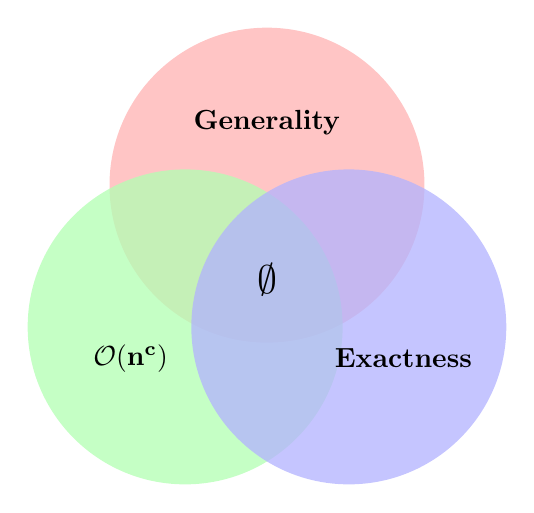
\begin{tikzpicture}
        \begin{scope}[blend mode = normal,opacity=0.75]
            \fill[red!30!white]   ( 90:1.2) circle (2);
            \fill[green!30!white] (210:1.2) circle (2);
            \fill[blue!30!white]  (330:1.2) circle (2);
        \end{scope}
        \node at ( 90:2)    {\textbf{Generality}};
        \node at ( 210:2)   {$\mathbf{\mathcal{O}(n^c)}$};
        \node at ( 330:2)   {\textbf{Exactness}};
        \node [font=\Large] {$\emptyset$};
    \end{tikzpicture}
\end{center}


\begin{definition}[Parametrized Problem{\cite[Def 1.1]{Cygan2015}}]
    A parametrized problem is a $L\subseteq\Sigma^*\times \mathbb{N}$ ($\Sigma$ finite fixed alphabet) for an instance $(x,k)\in \Sigma^*\times \mathbb{N}$, where k is called the \textit{parameter}.
\end{definition}

\begin{definition}[Instance Size]
    The \textbf{size of an instance} of an instance $(x,k)$ of a parametrized problem is $\abs{(x,k)} = \abs{x} + k$
\end{definition}
We will now clarify the basic terminology withing Parametrized Complexity. 
We are now giving a short introduction into the world of parametrized complexity. 
* General Introduction


\subsection{Fixed Parameter Tractability}

\begin{definition} [The Class FPT {\cite[Def 1.2]{Cygan2015}}]
    A parametrized problem $L\subseteq\Sigma^*\times\mathbb{N}$ is called \textit{fixed-parameter tractable} if there exists an algorithm A (called a \textit{fixed-parameter algorithm}), a computable function $f:\mathbb{N} \rightarrow \mathbb{N}$ and a constant c such that, given $(x,k) \in \Sigma^* \times \mathbb{N}$, the algorithm $\mathcal{A}$ correctly decides whether $(x,k) \in L$ in time bounded by $f(k) \cdot |(x,k)|^c$. The complexity class containing all fixed-parameter tractable problems is called \textit{FPT}
\end{definition}


\subsection{Kernelization}

\begin{definition}[kernelization Algoritm{\cite[Def 2.1]{Cygan2015}}]
A \textit{Kernelization Algorithm} or \textit{kernel} is an algorithm $\mathfrak{A}$ for a parametrized Problem Q, that given an instance $(I,k)$ of Q works in polynomial time and returns an equivalent instance $(I', k')$ of Q. Moreover, we require that $size_{\mathfrak{A}}(k) \leq g(k)$ for some computable function $g:\mathbb{N} \rightarrow \mathbb{N}$
\end{definition}

%TODO better
If we bound the size of the kernel by linear function $f(m) = \mathcal{O}(k)$, we say that the problem admits a \textbf{linear kernel}. 

%Examplary, if we reduce a graph for a graph problem in such a way that we can garuantee that our reduced graph only has a a few vertices \textbf{linear} in  $k$ left

The main idea, preprocessing algorithm, shrink size as much as possible, sound reduction rules,small output instance

\begin{definition}[Output size of a Preprocessing Procedure {\cite[p. 18]{Cygan2015}}] The output size of a preprocessing algorithms $\mathfrak{A}$ is defined as 

    \[\mathrm{size}_{\mathfrak{A}}(k) = \sup\{\abs{I'} + l': (I',k')= \mathfrak{A}(I,k), I \in \Sigma^* \} \]
\end{definition}

possibly infinite

Clearly, if there exists a kernelization algorithm for a problem $L$ and an algorithm $\mathfrak{A}$ with any runtime to decide $L$, the problem is in $FPT$ because after the kernelization pre-processing has been applied, the size of the reduced instance is a function merely in $k$ and independent of the input size $n$. In \cref{ch:linkern} we will explicitly construct a kernel for \psdom and hence showing it to be in \textit{FPT}. 

% Interstingly, als the converse?

\begin{definition}[Reduction Rules {\cite[p. 18]{Cygan2015}}]
A \textbf{reduction rule} is a function $\phi:\Sigma^* \times \mathbb{N} \rightarrow \Sigma^* \times \mathbb{N}$ that maps an instance $(x,k)$ to an equivalent instance $(x',k')$ such that $phi$ is computable in time polynomial in $\abs{x}$ and $k$
\end{definition}

\begin{definition}[Equivalent Instance {\cite[p. 18]{Cygan2015}}]
     This is a test
\end{definition}

\begin{definition}{Soundness of a rule}

\end{definition}

A \textbf{reduction rule} is a function $\Sigma* \times \mathbb{N}$ that maps an instance $(x,k)$ to an equivalent instance $(x',k')$ such that xx is computable in time polynomial in $\abs{x}$ and $k$

\subsection{Fixed Parameter Intractability: The w-Hierarchy}
\subsection{Compare to classical NP-Hardness theory}

\subsubsection{Parametrized Reductions}
\begin{definition}[Parametrized Reduction {\cite[Def 13.1]{Cygan2015}}] Let $A,B\subseteq \Sigma^*\times\mathbb{N}$ two parametrized problems. A \textit{Parametrized Reduction} from A to B is an algorithm that, given an instance $(x,k)$ of A, outputs an instance $(x', k')$ of B such that

    \begin{itemize}
        \item $(x,k)$ is a \textcolor{gray}{yes instance} of A \textbf{iff} $(x',k')$ is a \textcolor{gray}{yes instance} of B
        \item $k' \leq g(k)$ for some computable function $g$
        \item the running time is $f(k)\cdot |x|^{\mathcal{O}(1)}$ (FPT!)
    \end{itemize}
\end{definition}
    \subsubsection{The $w$-hierarchy}



\section{The Domination Problem}

\begin{prb}[DOMINATING SET {\cite[p. 586]{Cygan2015}}]{prb:ds}
    \begin{tabularx}{0.9\textwidth}{>{\hsize=0.30\hsize}X>{\hsize=0.8\hsize}X}
        \textbf{Input:} & Graph \G and an integer $k$\\
        \textbf{Question:} & Is there a set $X \subseteq V$ of size at most $k$ such that $N[X] = V$? \\
    \end{tabularx}
\end{prb}


Goddard, Henning and McPiallan a

\begin{prb}[SEMITOTAL DOMINATING SET {\cite{Goddard2014}}]{prb:tds}
    
    \begin{tabularx}{0.8\textwidth}{>{\hsize=0.35\hsize}X>{\hsize=0.8\hsize}X}
        \textbf{Input:} & Graph \G and an integer $k$\\
        \textbf{Question:} & Is there a subset $X \subseteq V$ of size at most $k$ such that $N[X] = V$ and for all $d_1 \in X$ there exists another $d_2 \in X$ such that $d(d_1, d_2) \leq 2$?\\
    \end{tabularx}
        
\end{prb}

\begin{prb}[TOTAL DOMINATING SET {\cite[p. 596]{Cygan2015}}]{prb:sds}
    \begin{tabularx}{0.8\textwidth}{>{\hsize=0.35\hsize}X>{\hsize=0.8\hsize}X}
        \textbf{Input:} & Graph \G and an integer $k$\\
        \textbf{Question:} & Does there exists a set $X \subseteq V$ of at most $k$ vertices of G such that for every $u \in V(G)$ there exists $v \in X$ with $\{u,v\} \in E$ \\
    \end{tabularx}
        
\end{prb}





Dominating Set

Semitotal Dominating Set

Total Dominating Set

we denote y as the dominating number. Clearly $y_t < y_s < y_d$.
Notatio of an independent set
\subsection{Preliminaries}

* Witness
* u pendant ofrom a vertex c if $N(u) = \{w\}$
* domination 

Let $D$ be a dominating set of G and $w \in V(G) \setminus D$. For any neighbor $v \in D \cap N(w)$, we say that $d_1$ \textit{dominates} $w$ For two dominating vertices $d_1, d_2in D$. If 

\sdom

%\subsection{Some useful notation}


Definition, dominating number

\section{Complexity Status of \sdom}\label{ch:complexity-status}

\section{\hmath $w[i]$-Intractibility}

Now some w[i] hard classes. 

\subsection{Warm-Up: \hmath $W[2]$-hard on General Graphs}

% TODO can we conclude anything for AT Free Graphs?
%% TODO Extend to r-partite

As any \bg with bipartition can be split further into \rpg this results also implies the \wone-hardness of \rpg

